% base-article.tex -- canonical, end-to-end compilable article skeleton.
% Compile from this directory (priv/latex/templates/) with:
%   tectonic base-article.tex
% The author copies this file, then adjusts \LatexLibRoot if it moves elsewhere
% (set it to the absolute or relative path of priv/latex/, WITH a trailing slash).

\documentclass[11pt,a4paper]{article}

% Root of the LaTeX library (path to priv/latex/, trailing slash required).
\providecommand{\LatexLibRoot}{../}
% article.tex -- modern article preamble.
% Compiles clean under tectonic and pdflatex (uses fontenc[T1]+lmodern, not fontspec).
% Usage: after \documentclass{article}, \input this file, then \input macros.
%   \documentclass[11pt,a4paper]{article}
%   % article.tex -- modern article preamble.
% Compiles clean under tectonic and pdflatex (uses fontenc[T1]+lmodern, not fontspec).
% Usage: after \documentclass{article}, \input this file, then \input macros.
%   \documentclass[11pt,a4paper]{article}
%   % article.tex -- modern article preamble.
% Compiles clean under tectonic and pdflatex (uses fontenc[T1]+lmodern, not fontspec).
% Usage: after \documentclass{article}, \input this file, then \input macros.
%   \documentclass[11pt,a4paper]{article}
%   \input{../preambles/article.tex}   % or an absolute/relative path
% This file loads ../macros.tex at the end, so callers get macros for free.

% --- Encoding & fonts (pdflatex + tectonic compatible) --------------------
\usepackage[T1]{fontenc}
\usepackage[utf8]{inputenc}
\usepackage{lmodern}
\usepackage{microtype}

% --- Page geometry --------------------------------------------------------
\usepackage[margin=1in]{geometry}

% --- Math -----------------------------------------------------------------
\usepackage{amsmath}
\usepackage{amssymb}
\usepackage{amsthm}
\usepackage{mathtools}

% --- Graphics, tables, units, color --------------------------------------
\usepackage{graphicx}
\usepackage{tikz}
\usepackage{booktabs}
\usepackage{siunitx}
\usepackage{xcolor}

% --- Language & quotes ----------------------------------------------------
\usepackage{csquotes}

% --- Hyperlinks (load hyperref last, before any macros that need it) ------
\usepackage{hyperref}
\definecolor{linknavy}{RGB}{0,51,102}
\hypersetup{
  colorlinks=true,
  linkcolor=linknavy,
  citecolor=linknavy,
  urlcolor=linknavy,
  filecolor=linknavy,
  pdfborder={0 0 0},
  bookmarksnumbered=true,
}

% --- Shared macros --------------------------------------------------------
\input{\LatexLibRoot macros.tex}
   % or an absolute/relative path
% This file loads ../macros.tex at the end, so callers get macros for free.

% --- Encoding & fonts (pdflatex + tectonic compatible) --------------------
\usepackage[T1]{fontenc}
\usepackage[utf8]{inputenc}
\usepackage{lmodern}
\usepackage{microtype}

% --- Page geometry --------------------------------------------------------
\usepackage[margin=1in]{geometry}

% --- Math -----------------------------------------------------------------
\usepackage{amsmath}
\usepackage{amssymb}
\usepackage{amsthm}
\usepackage{mathtools}

% --- Graphics, tables, units, color --------------------------------------
\usepackage{graphicx}
\usepackage{tikz}
\usepackage{booktabs}
\usepackage{siunitx}
\usepackage{xcolor}

% --- Language & quotes ----------------------------------------------------
\usepackage{csquotes}

% --- Hyperlinks (load hyperref last, before any macros that need it) ------
\usepackage{hyperref}
\definecolor{linknavy}{RGB}{0,51,102}
\hypersetup{
  colorlinks=true,
  linkcolor=linknavy,
  citecolor=linknavy,
  urlcolor=linknavy,
  filecolor=linknavy,
  pdfborder={0 0 0},
  bookmarksnumbered=true,
}

% --- Shared macros --------------------------------------------------------
\input{\LatexLibRoot macros.tex}
   % or an absolute/relative path
% This file loads ../macros.tex at the end, so callers get macros for free.

% --- Encoding & fonts (pdflatex + tectonic compatible) --------------------
\usepackage[T1]{fontenc}
\usepackage[utf8]{inputenc}
\usepackage{lmodern}
\usepackage{microtype}

% --- Page geometry --------------------------------------------------------
\usepackage[margin=1in]{geometry}

% --- Math -----------------------------------------------------------------
\usepackage{amsmath}
\usepackage{amssymb}
\usepackage{amsthm}
\usepackage{mathtools}

% --- Graphics, tables, units, color --------------------------------------
\usepackage{graphicx}
\usepackage{tikz}
\usepackage{booktabs}
\usepackage{siunitx}
\usepackage{xcolor}

% --- Language & quotes ----------------------------------------------------
\usepackage{csquotes}

% --- Hyperlinks (load hyperref last, before any macros that need it) ------
\usepackage{hyperref}
\definecolor{linknavy}{RGB}{0,51,102}
\hypersetup{
  colorlinks=true,
  linkcolor=linknavy,
  citecolor=linknavy,
  urlcolor=linknavy,
  filecolor=linknavy,
  pdfborder={0 0 0},
  bookmarksnumbered=true,
}

% --- Shared macros --------------------------------------------------------
\input{\LatexLibRoot macros.tex}


\title{A Compile-Ready Article Skeleton}
\author{OSA \LaTeX{} Author}
\date{\today}

\begin{document}
\maketitle

\begin{abstract}
This skeleton demonstrates the house style: display math with \verb|\[...\]|
and \texttt{align}, \texttt{booktabs} tables, a figure placeholder, and the
shared macros from \texttt{macros.tex}. It compiles cleanly under \texttt{tectonic}.
\end{abstract}

\section{Introduction}
\label{sec:intro}
Let $f\colon \R \To \R$ be continuous. For any $x \in \R$ we write $\abs{x}$ for
its absolute value and $\norm{x}$ for a norm on $\R^n$. Display math uses
\verb|\[...\]| or \texttt{align}:
\[
  \int_{a}^{b} f(x)\,\dd{x} = \eval{F(x)}{a}{b},
\]
and multi-line derivations use \texttt{align}:
\begin{align}
  (a + b)^2 &= a^2 + 2ab + b^2, \label{eq:square}\\
  \deriv{}{x}\, e^{x} &= e^{x}.
\end{align}

\begin{theorem}[Fundamental bound]
\label{thm:bound}
For every $x \in \R$, $\abs{x} \ge 0$, with equality iff $x = 0$.
\end{theorem}

\begin{proof}
Immediate from the definition of the absolute value.
\end{proof}

\section{A Table}
\label{sec:table}
Table~\ref{tab:results} uses \texttt{booktabs} rules (never \verb|\hline|) and
\texttt{siunitx} for aligned numbers.

\begin{table}[htbp]
  \centering
  \caption{Illustrative results.}
  \label{tab:results}
  \begin{tabular}{l S[table-format=3.2] S[table-format=1.3]}
    \toprule
    Method & {Score} & {Error} \\
    \midrule
    Baseline & 87.40 & 0.120 \\
    Proposed & 94.25 & 0.031 \\
    \bottomrule
  \end{tabular}
\end{table}

\section{A Figure}
\label{sec:figure}
Figure~\ref{fig:placeholder} is a placeholder drawn with \texttt{tikz} so the
skeleton compiles without any external image file. Replace it with
\verb|\includegraphics{...}| once a real asset exists.

\begin{figure}[htbp]
  \centering
  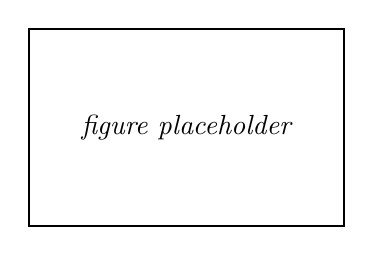
\begin{tikzpicture}
    \draw[thick] (0,0) rectangle (4,2.5);
    \node at (2,1.25) {\itshape figure placeholder};
  \end{tikzpicture}
  \caption{Placeholder figure.}
  \label{fig:placeholder}
\end{figure}

Cross-references (Section~\ref{sec:intro}, Theorem~\ref{thm:bound},
Equation~\eqref{eq:square}) resolve through \texttt{hyperref}.

\end{document}
